\documentclass{beamer}
\usepackage[utf8]{inputenc}
\usepackage[russianb]{babel}
\usepackage{graphicx}
\usepackage{subfig}
\graphicspath{ {./pics/} }

\title{Применение нейроных сетей для моделирования систем управления}
\author{Сивков Антон Александрович\\
{\footnotesize научный руководитель: д.ф.--м.н., профессор Фомичев В. В.}\\
}
\institute{
{\footnotesize
Кафедра нелинейных динамических систем и процессов управления\\
Факультет вычислительной математики и кибернетики\\
Московский государственный университет имени М.В. Ломоносова\\
}
}
\date{\the\year}

\begin{document}
\frame{\titlepage}
 
\begin{frame}
\frametitle{Постановка задачи}
\begin{itemize}
\item Решается задача идентификации
\item Объект моделируется как 'чёрный ящик'
\item Сеть обучается предсказывать выходные сигналы объекта управления по входным
\item Сравнивается способность сетей с различными архитектурами экстраполировать поведение объекта. Такое моделирование не всегда корректно, однако позволяет сравнивать качество моделирования без использования сложных нелинейных объектов.
\end{itemize}
Объект управления, использованный для моделирования:\\
\begin{equation}
\centering
H = \frac{z}{(z-\frac{1}{2})(z-\frac{1}{3})(z-\frac{1}{4})},~dt=1~sec.,~x_{0}=0
\end{equation}
\end{frame}

\begin{frame}{Многослойный перцептрон}
\begin{figure}[h]
    \centering
    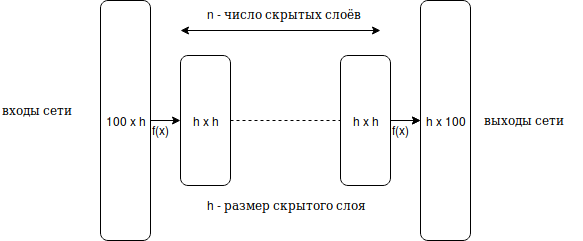
\includegraphics[width=0.7\textwidth]{multi_layer_perceptron}
    \caption{Схема многослойного перцептрона}
\end{figure}
Размер скрытого слоя h, число скрытых слоев n, функция активации f(x) --- гиперпараметры
\end{frame}

\begin{frame}{Эксперимент с многослойным перцептроном}
\begin{figure}[!ht]
     \subfloat[Предсказание при отсутствии сдвига частот]{%
         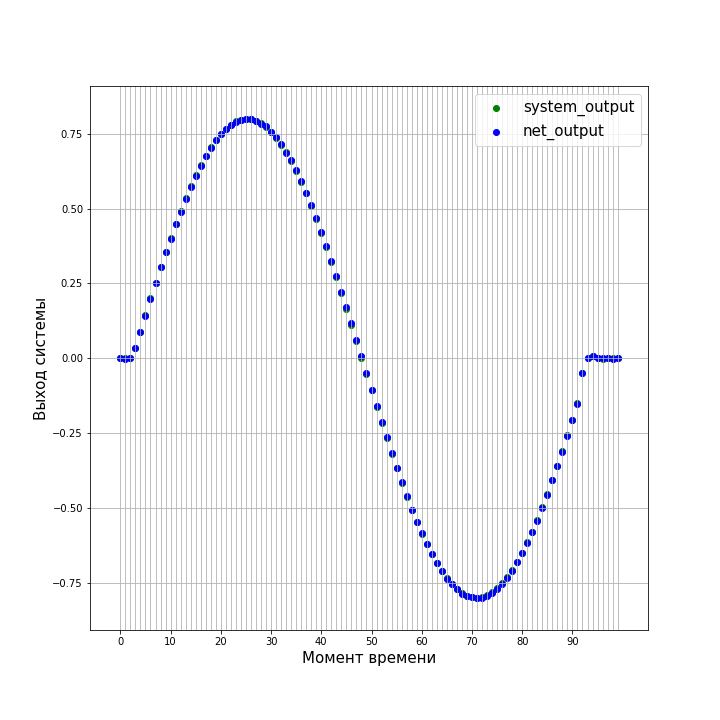
\includegraphics[width=0.45\textwidth]{fcnet_prediction}
     }
     \hfill
     \subfloat[Предсказание при сдвиге частоты на 0.1 Гц (частота 0.2 Гц)]{%
         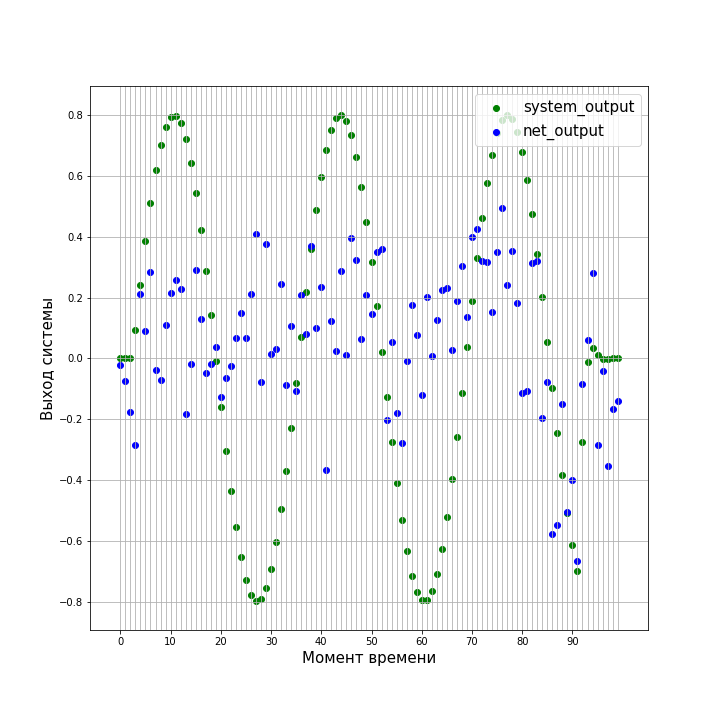
\includegraphics[width=0.45\textwidth]{fcnet_prediction_shifted}
     }
     \caption{Предсказание поведения объекта}
     \label{fig:dummy}
\end{figure} 
\end{frame}

\begin{frame}{Выводы для многослойного перцептрона}
\begin{itemize}
\item Сеть неспособна экстраполировать поведение объекта. Среднеквадратичная ошибка при сдвиге частот $\approx 0.2$. Перебор гиперпараметров сети не даёт существенных улучшений. 
\item В статьях по теме идентификации систем с помощью многослойного перцептрона решают задачи идентификации для сложных нелинейных объектов без тестирования способности сети к экстраполяции. 
\end{itemize}
\end{frame}

\begin{frame}{Сеть с долгосрочно--краткосрочной памятью (LSTM)}
\begin{figure}[h]
    \centering
    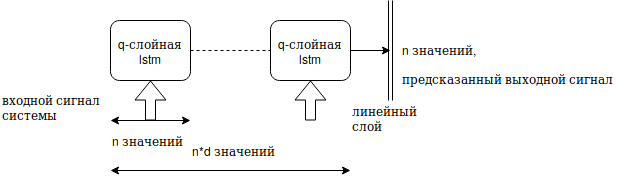
\includegraphics[width=0.7\textwidth]{rnn}
    \caption{Схема основанной на lstm ячейке сети}
\end{figure}
Размер шага рекурсии, входа и выхода ячейки n, максимальная глубина рекурсии d, число внутренних слоев ячейки q --- гиперпараметры. 
\end{frame}

\begin{frame}{Эксперимент с lstm сетью}
\begin{figure}[!ht]
     \subfloat[Предсказание при сдвиге частоты на 0.1 Гц (частота 0.2 Гц)]{%
         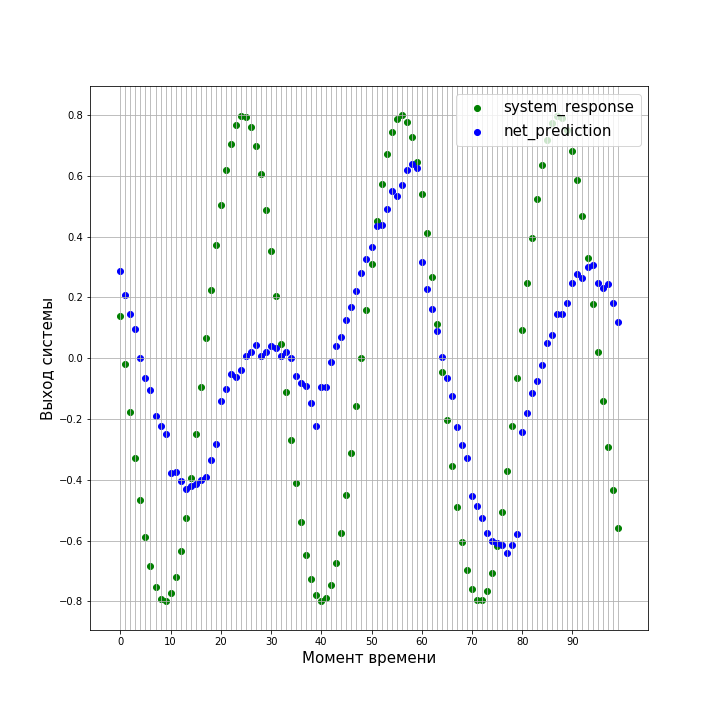
\includegraphics[width=0.45\textwidth]{rnn_prediction_shifted}
     }
     \hfill
     \subfloat[Предсказание при подаче на вход сети смеси сигналов с частотой 0.1 Гц и 0.2 Гц]{%
         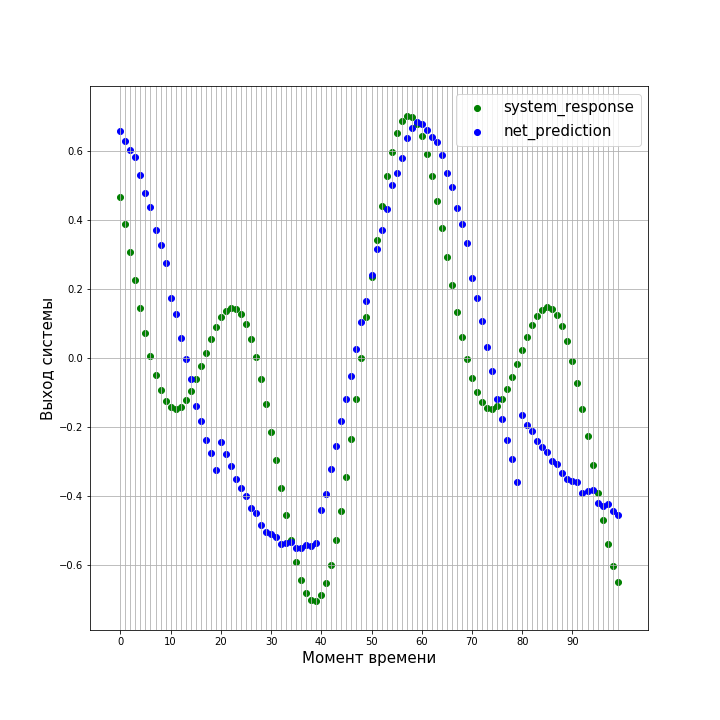
\includegraphics[width=0.45\textwidth]{rnn_prediction_mix}
     }
     \caption{Предсказание поведения объекта}
     \label{fig:dummy}
\end{figure}
\end{frame}

\begin{frame}
\begin{figure}[h]
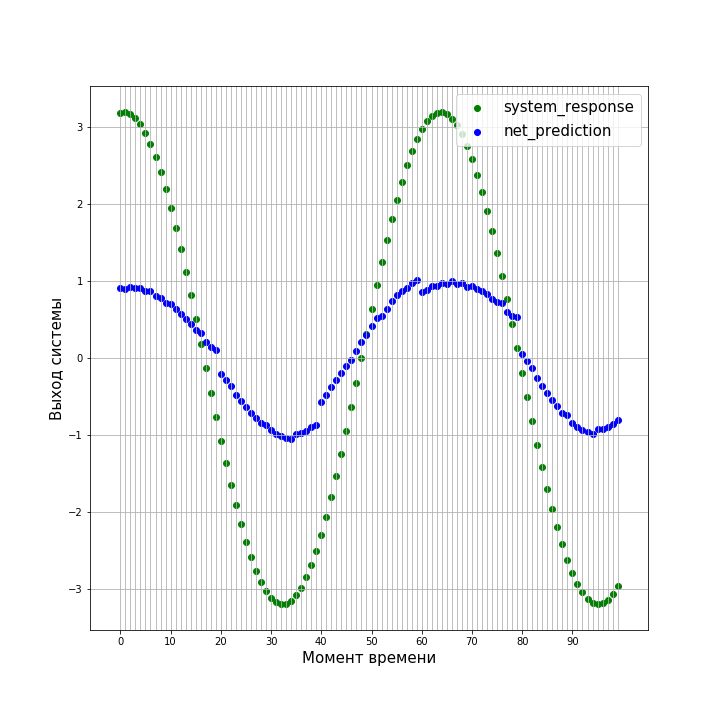
\includegraphics[width=0.7\textwidth]{rnn_prediction_high_magnitude}
\caption{Предсказание при увеличенной амплитуде сигнала}
\end{figure}
\end{frame}

\begin{frame}{Выводы для lstm сети}
\begin{itemize}
\item Сеть допускает значительные ошибки, однако среднеквадратичная ошибка предсказания уменьшается на порядок по сравнению с многослойным перцептроном. Среднеквадратичная ошибка при сдвиге частот $\approx 0.02$
\item Интересен тот факт, что с наращиванием сложности сети с помощью гиперпараметров, ошибка на смещённой выборке \textbf{возрастает практически монотонно}. 
\item Идея использования lstm для идентификации встречается в статьях, однако исследования способности сетей к экстраполяции затруднительно найти.
\end{itemize}
\end{frame}

\begin{frame}{lstm сеть, использующая данные выхода системы для предсказания}
\begin{figure}[h]
    \centering
    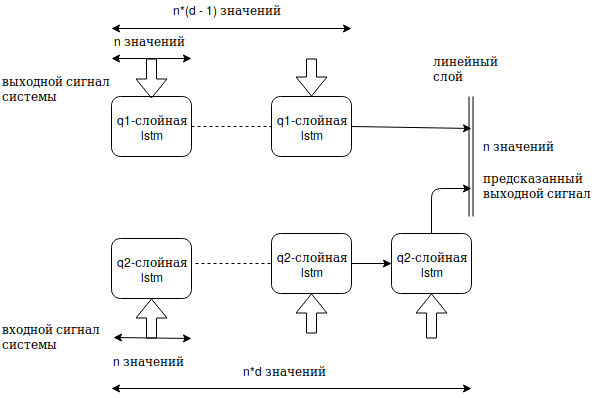
\includegraphics[width=0.6\textwidth]{updated_rnn}
    \caption{Схема основанной на lstm ячейке сети, использующей выходной сигнал системы}
\end{figure}
Размер шага рекурсии, входа и выхода ячейки n, максимальная глубина рекурсии d, количество внутренних слоев ячеек q1 и q2 --- гиперпараметры.
\end{frame}

\begin{frame}
\begin{figure}[!ht]
     \subfloat[Предсказание при сдвиге частоты на 0.1 Гц (частота 0.2 Гц)]{%
         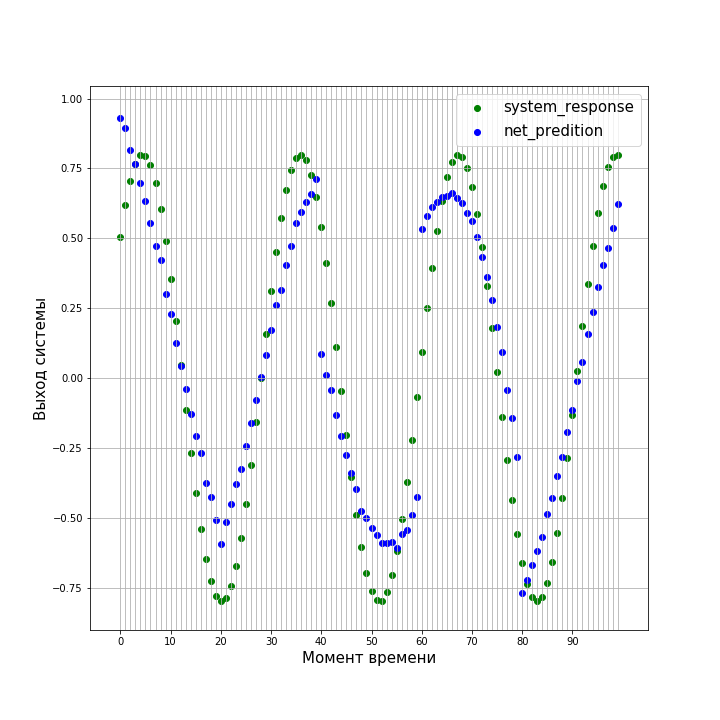
\includegraphics[width=0.45\textwidth]{rnn_2_prediction_shifted}
     }
     \hfill
     \subfloat[Предсказание при подаче на вход сети смеси сигналов с частотой 0.1 Гц и 0.2 Гц]{%
         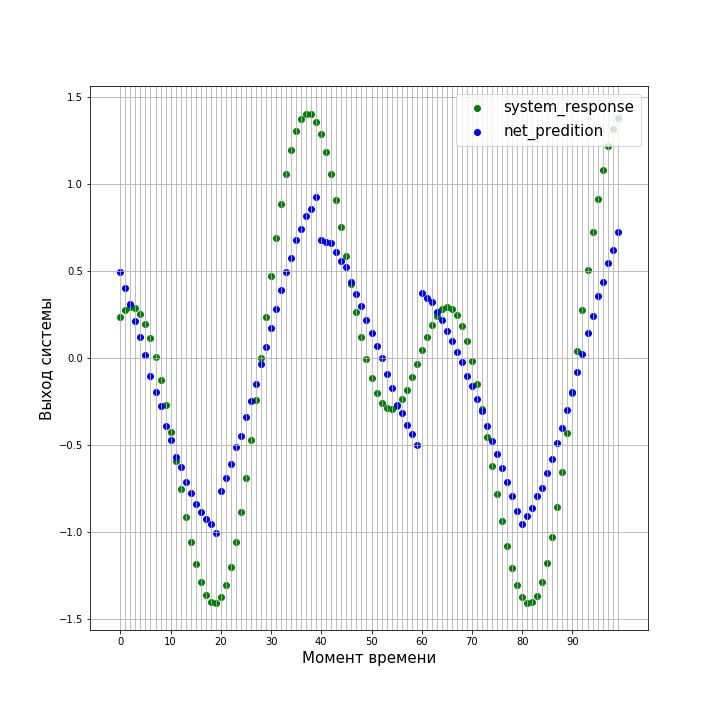
\includegraphics[width=0.45\textwidth]{rnn_2_prediction_mix}
     }
     \caption{Предсказание поведения объекта}
     \label{fig:dummy}
\end{figure}
\end{frame}

\begin{frame}{Выводы для улучшенной lstm сети}
\begin{itemize}
\item Сеть, использующая собственные предсказания на предыдущих моментах времени как входные данные, предсказывает выход существенно лучше, чем сеть, использующая только входные сигналы. Среднеквадратичная ошибка при сдвиге частот $\approx 0.012$.
\item Наблюдается аналогичный предылущему случаю эффект возрастания ошибки на смещенной выборке при росте сложности сети.
\item Идея использования предсказаний в предыдущие моменты времени для следующих встречается в одной из тематических статей, однако такой подход широко используется в различных задачах, решаемых с помощью нейронных сетей.
\end{itemize}
\end{frame}

\begin{frame}{Выводы}
\begin{itemize}
\item Проведен сравнительный анализ различных архитектур сетей, однозначно выявлены сети, обладающие лучшей способностью к экстраполяции поведения объекта управления.
\item Определен примерный вектор дальнейшего поиска наиболее адекватной задаче архитектуры сети, а именно: сеть должна быть реккурентной; должна использовать предсказания выхода  объекта управления в предыдущие моменты времени как входы; не должна обладать чрезмерным количеством параметров во избежание переобучения.
\end{itemize}
\end{frame}

\begin{frame}
\centering
Спасибо за внимание
\end{frame}

\end{document}
